\section{結果}
\subsection{ストレッチセンサ計測精度評価}
Fig. \ref{output_for_test}のような出力を各空気圧人工筋に与えた結果,
Table.\ref{strain}のような長さの結果となった.
また,それぞれの時におけるストレッチセンサ時定数の結果を求めると,Table.\ref{4_2}に示す様になった.
\begin{table}[h]
    \caption{ストレッチセンサ 長さ(mm) 計測結果}
    \label{strain}
    \begin{center}
        \begin{tabular}{|c|c|ccc|}\hline
            \multicolumn{2}{|c|}{} & \multicolumn{3}{c|}{筋肉種類}\\
            \cline{3-5}
            \multicolumn{2}{|c|}{} & 前脛骨筋 & 腓骨筋 & ヒラメ筋 \\ \hline
            & 1 & 244 & 196 & 209 \\ \cline{2-5}
            & 2 & 243 & 194 & 208 \\ \cline{2-5}
            & 3 & 242 & 192 & 209 \\ \cline{2-5}
            & 4 & 239 & 194.5 & 212 \\ \cline{2-5}
            & 5 & 211 & 202 & 217 \\ \cline{2-5}
            計測位置 & 6 & 207.5 & 219 & 235 \\ \cline{2-5}
            & 7 & 206.7 & 220 & 234 \\ \cline{2-5}
            & 8 & 211 & 222 & 236 \\ \cline{2-5}
            & 9 & 207.8 & 206.8 & 219 \\ \cline{2-5}
            & 10 & 238 & 195 & 208.8 \\ \cline{2-5}
            & 11 & 242 & 192.4 & 207.8 \\ \cline{2-5}
            & 12 & 244 & 191.4 & 206.2 \\ \hline
        \end{tabular}
    \end{center}
\end{table}

\newpage

%セルを結合して中央揃え
%(参考):https://qiita.com/ta_b0_/items/c8c828b6a53d49498736
\begin{table}[h]
    \caption{ストレッチセンサ 時定数(us) 計測結果}
    \label{4_2}
        \begin{center}
            \begin{tabular}{|c|c|ccc|}\hline
            \multicolumn{2}{|c|}{} & \multicolumn{3}{c|}{筋肉種類}\\
            \cline{3-5}
            \multicolumn{2}{|c|}{} & 前脛骨筋 & 腓骨筋 & ヒラメ筋 \\ \hline
            & 1 & 45.911±0.004 & 69.987±0.001 & 55.856±0.004 \\ \cline{2-5}
            & 2 & 46.222±0.005 & 69.781±0.004 & 55.586±0.005 \\ \cline{2-5}
            & 3 & 46.233±0.004 & 69.869±0.005 & 55.663±0.006 \\ \cline{2-5}
            & 4 & 45.780±0.005 & 69.989±0.005 & 55.518±0.007 \\ \cline{2-5}
            & 5 & 47.974±0.002 & 69.068±0.005 & 54.599±0.007 \\ \cline{2-5}
            計測位置 & 6 & 48.797±0.004 & 68.485±0.006 & 52.699±0.006 \\ \cline{2-5}
            & 7 & 48.947±0.003 & 69.259±0.006 & 52.855±0.006 \\ \cline{2-5}
            & 8 & 48.926±0.003 & 69.206±0.017 & 52.539±0.007 \\ \cline{2-5}
            & 9 & 49.028±0.003 & 69.546±0.007 & 55.451±0.007 \\ \cline{2-5}
            & 10 & 46.109±0.003 & 70.017±0.007 & 56.660±0.006 \\ \cline{2-5}
            & 11 & 46.099±0.005 & 70.174±0.008 & 56.554±0.007 \\ \cline{2-5}
            & 12 & 47.001±0.004 & 68.908±0.010 & 55.638±0.006 \\ \hline
        \end{tabular}
    \end{center}
\end{table}

\section{考察}
\subsection{ストレッチセンサ計測精度}
先ほどの結果より,それぞれの計測位置における空気圧人工筋の長さをグラフに表すと,
Fig.\ref{4-ml}の様になった.このグラフから見てわかるように,腓骨筋とヒラメ筋が組となって
前脛骨筋と逆位相のsin波形的動きをさせることが出来た.今回,足関節ロボットの空気圧人工筋
それぞれに対して,Fig.\ref{output_for_test}の出力を出すよう指令を与えたので
システムとして問題なく動いたことがわかる.

\begin{figure}[h]
    \begin{center}
        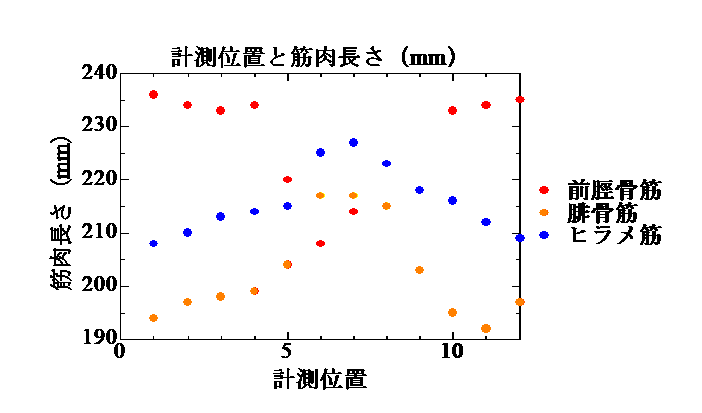
\includegraphics[width=0.78\columnwidth,clip]{4_consideration/ml.eps}
    \end{center}
    \caption{計測位置と各空気圧人工筋の長さの関係}
    \label{4-ml}
\end{figure}

\newpage

続いて,Table.\ref{4_2}の結果を用いて,横軸にセンサの長さ,縦軸に時定数としたグラフを
描画すると,Fig.\ref{ml-rc1},\ref{ml-rc2},\ref{ml-rc3}に示すようになった.
各筋肉に関して,長さが増加するとセンサでの計測値が減少した.
どの筋肉においても同様の結果を示しており,ストレッチセンサが伸びると
静電容量が減少するといったことが分かった.

一方でセンサごとに空気圧人工筋の長さに対する計測値の変化の特性が異なる.これは,
センサ自体が自作されており,その製作時のむらによるものだと考えられる.それに加えて,
空気圧人工筋に設置する時にある程度テンションを与えて設置するのだが,そのテンションの
かけ方具合にもよると考えられる.実際に使用するときは,ストレッチセンサを空気圧人工筋に
設置した状態で,今回の実験の様にセンサ特性の解析を行う必要があると考えられる.

また,空気圧人工筋の伸びの変化に対して,時定数の変化が非常に微小なものとなっている.
今回の時定数の結果や,製作したRC回路の抵抗値$1.5M\Omega$より静電容量の変化量に関して考えると,
最も変化が大きかったヒラメ筋においても$35~38pF$の変化しか現れなかった.
これに対する対策として,RC回路における抵抗値の再選定を行う必要があると考えられた.
抵抗値を増加させると時定数も増加するのでマイコンで変化量を計測しやすくなる.
一方で,抵抗値を増大させると計測ノイズ成分も大きくなるので,その辺りも踏まえて抵抗値の
再選定をしていく必要があると考えられる.

\begin{figure}[h]
    \begin{center}
        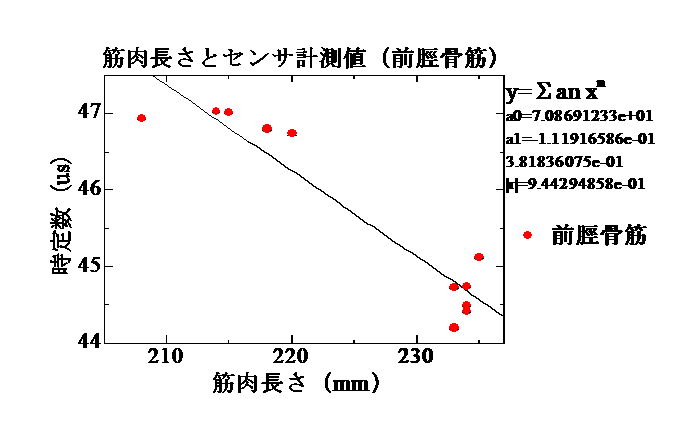
\includegraphics[width=0.78\columnwidth,clip]{4_consideration/zenkei.eps}
    \end{center}
    \caption{空気圧人工筋の長さとセンサ計測値の関係(前脛骨筋)}
    \label{ml-rc1}
\end{figure}

\begin{figure}[h]
    \begin{center}
        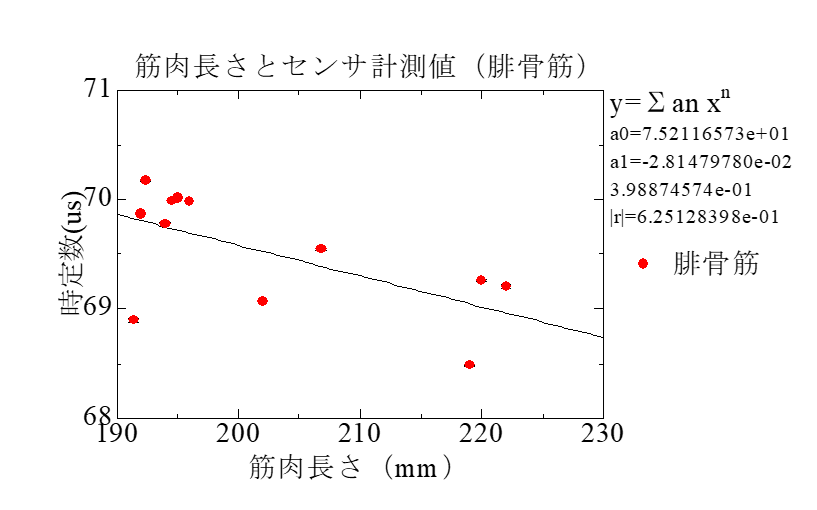
\includegraphics[width=0.78\columnwidth,clip]{4_consideration/hikotsu.eps}
    \end{center}
    \caption{空気圧人工筋の長さとセンサ計測値の関係(腓骨筋)}
    \label{ml-rc2}
\end{figure}

\begin{figure}[h]
    \begin{center}
        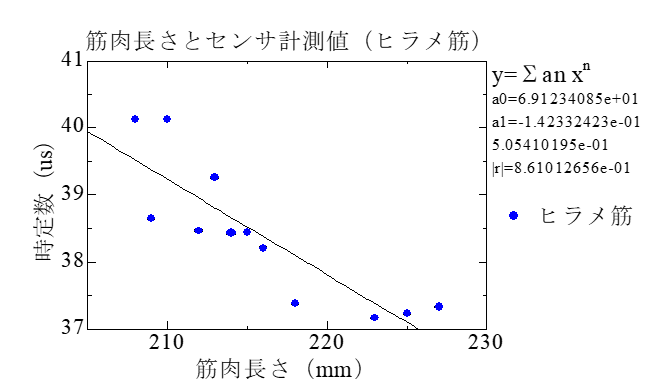
\includegraphics[width=0.78\columnwidth,clip]{4_consideration/hirame.eps}
    \end{center}
    \caption{空気圧人工筋の長さとセンサ計測値の関係(ヒラメ筋)}
    \label{ml-rc3}
\end{figure}